\begin{question}
\noindent Triangle $M$ has vertices at $A(1,1)$, $B(3,1)$ and $C(1,2)$.

\noindent Enlarge triangle $M$ by scale factor $-2$, centre $(0,0)$.

\begin{center}
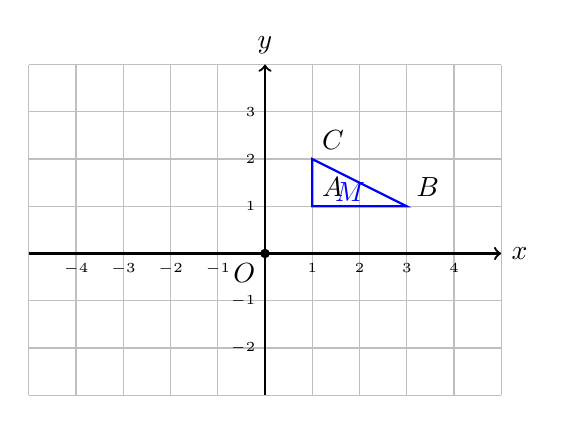
\begin{tikzpicture}[scale=0.6]
    % Grid
    \draw[step=1cm, lightgray, thin] (-5,-3) grid (5,4);
    % Axes
    \draw[thick,->] (-5,0) -- (5,0) node[right] {$x$};
    \draw[thick,->] (0,-3) -- (0,4) node[above] {$y$};
    % Axis labels
    \foreach \x in {-4,-3,-2,-1,1,2,3,4}
        \node[below] at (\x,0) {\tiny $\x$};
    \foreach \y in {-2,-1,1,2,3}
        \node[left] at (0,\y) {\tiny $\y$};
    % Triangle M
    \draw[thick, blue] (1,1) -- (3,1) -- (1,2) -- cycle;
    \node[above right] at (1,1) {$A$};
    \node[above right] at (3,1) {$B$};
    \node[above right] at (1,2) {$C$};
    \node[blue] at (1.8,1.3) {$M$};
    % Centre of enlargement
    \filldraw[black] (0,0) circle (2.5pt);
    \node[below left] at (0,0) {$O$};
\end{tikzpicture}
\end{center}

\noindent On the grid, draw the image of triangle $M$ after this enlargement. Label the image $M'$.

\vspace{6cm}

\begin{flushright}
    \answermarks{4}
\end{flushright}
\end{question}